\documentclass{beamer}

% Copyright 2010 Drow Ltd.
% 
% In principle, this file can be redistributed and/or modified under
% the terms of the GNU Public License, version 2.
% 
% However, this file is supposed to be a template to be modified
% for your own needs. For this reason, if you use this file as a
% template and not specifically distribute it as part of a another
% package/program, I grant the extra permission to freely copy and
% modify this file as you see fit and even to delete this copyright
% notice. 
\mode<presentation>
{
  \usetheme[titleline=true,
  alternativetitlepage=true,
  titlepagelogo=images/Java_logo]{Torino}
  \usecolortheme{nouvelle}
  \beamertemplatenavigationsymbolsempty
}

\usepackage{times}
\usepackage[utf8]{inputenc}
\usepackage[english,bulgarian]{babel}
\usepackage[T2A]{fontenc}

\usepackage{listings}
\lstset{language=Java,
  captionpos=b,
  tabsize=4,
  keywordstyle=\color{blue},
  commentstyle=\color{gray},
  stringstyle=\color{green},
  numbers=left,
  breaklines=true,
  showstringspaces=false,
  basicstyle=\ttfamily,
  emph={label},
  frame=shadowbox, 
  rulesepcolor=\color{blue},
  columns=fixed}

\title{Генерично програмиране}

\author{инж. Божидар ~Бацов}

\institute{Drow Ltd.}

\date{11.01.2011}

\subject{Talks}
% This is only inserted into the PDF information catalog. Can be left
% out. 

\begin{document}

\begin{frame}
  \titlepage
\end{frame}

\begin{frame}{Съдържание}
  \tableofcontents[pausesections]
\end{frame}

\section{Генерично програмиране}

\begin{frame}{Генерично програмиране}
  \begin{itemize}
  \item Въведено в Java 5
  \item Счита се от мнозина за най-голямата промяна в историята на
    Java
  \item Основната концепция е взаимствана от .NET, но реализацията е
    коренно различна
  \end{itemize}
\end{frame}

\begin{frame}{Анализ на нуждата от генерично програмиране}
  \transdissolve
  \begin{itemize}
  \item ArrayList
    \begin{itemize}
      \item клас от Collections API
      \item Динамично разширяем масив
      \item Предлага възможности като добавяне и изтриване на елемент,
        проверка за наличие на елемент и т.н.
    \end{itemize}
  \item Проблеми на негенеричната версия на ArrayList
    \begin{itemize}
      \item Обектите, които съдържа са от тип Object
      \item Необходими са преобразувания до типа, с който желаем да
        работим
      \item Няма ограничения на типа на обектите, които можем да
        поставим в ArrayList
      \item Сериозен потенциал за възникване на грешки по време на изпълнение
    \end{itemize}

  \end{itemize}
\end{frame}

\begin{frame}{Генерична версия ArrayList<T>}
  \transdissolve
  \begin{itemize}
  \item Декларацията на класа указва типа на неговите елементи
  \item Не са необходими преобразувания
  \item Не могат да бъдат добавени елементи от несъвместим тип
  \item Т - типова променлива(клас като String, Integer и т.н.)
  \end{itemize}
\end{frame}

\begin{frame}{Аспекти на генеричното програмиране}
  \transdissolve
  \begin{itemize}
  \item Използване на съществуващи генерични класове/методи
  \item Анализиране на проблеми в съществуващи генерични
    класове/методи
  \item Създаване на генерични класове/методи
  \end{itemize}
\end{frame}

\begin{frame}{Дефиниране на генеричен клас}
  \transdissolve
  \begin{itemize}
  \item Генеричния клас има в декларацията си
    една или повече типови променливи
   \item Типовите променливи се поставят в <>,
    след името на класа
   \item При инстанциране на класа ние
    заместваме типовите променливи с
    конкретни типове(String, Double, etc)
  \end{itemize}
\end{frame}

\begin{frame}[fragile]
  \frametitle{Дефиниране на генеричен клас - пример}
  \transdissolve
\begin{lstlisting}
class GenericClass<T> {
  private T someField;
  
  public T someMethod() {
  }
}

GenericClass<String> instance = new GenericClass<String>();
\end{lstlisting}
\end{frame}

\begin{frame}{Дефиниране на генеричен метод}
  \transdissolve
  \begin{itemize}
  \item   Може да дефинирате генерични методи
    в обикновени(негенерични) класове
   \item В декларацията на метод трябва трябва
    да добавите в <> генеричните типове
    преди връщата стойност от метода
   \item Когато извиквате генеричен метод може
    да поставите типовите променливи
    преди името на метода(но това
    обикновено не се налага)
  \end{itemize}
\end{frame}

\begin{frame}[fragile]
  \frametitle{Дефиниране на генеричен метод - пример}
  \transdissolve
\begin{lstlisting}
class SomeClass {
  public static <T> T someMethod(T param) {
  }
}

SomeClass.<String>someMethod("ala");
SomeClass.someMethod("bala");
\end{lstlisting}
\end{frame}

\begin{frame}{Граници(bounds) за типови променливи}
  \transdissolve
  \begin{itemize}
  \item Налагат ограничения на типовете, които могат да бъдат
    използвани с даден генеричен клас
  \item T extends Comparable
  \end{itemize}
\end{frame}

\begin{frame}{Генеричен код и виртуалната машина}
  \transdissolve
  \begin{itemize}
  \item В JVM няма концепция за генеричен клас
  \item Генеричните класове са имплементира изцяло като функционалност
    на компилатора
  \item Всеки генеричен клас има съответен суров клас(raw class) - в
    него типовете са изтрити и са заменени от техния ограничаващ тип
  \end{itemize}
\end{frame}

\begin{frame}{Генеричен код и JVM}
  \transdissolve
  \begin{itemize}
  \item Ако няма ограничаващ клас замяната е с Object
  \item Когато имаме повече от един тип –
    замяната с първия, а за другите
    компилатора добавя преобразувания в
    кода, където е необходимо
  \item \lstinline$class SomeClass<T extends Serializable & Comparable>$

  \end{itemize}
\end{frame}

\begin{frame}{Работа със стар код(преди Java 5)}
  \transdissolve
  \begin{itemize}
  \item Предупреждения при използване на сурови класове
  \item Потискане на предупреждения на несигурни операции
    \begin{itemize}
      \item Анотация @SuppressWarnings("`Unchecked"')
    \end{itemize}

  \end{itemize}
\end{frame}

\begin{frame}{Ограничения}
  \transdissolve
  \begin{itemize}
  \item Типов параметър не може да бъде примитивен тип
  \item Губи се информацията за типа по време на изпълнение
  \item Не могат да се създават масиви от генерични типове
  \item Не може да инстанциране типови променливи
  \item Типовите променливи не са позволени в статичен контекст
  \item Могат да възникнат конфликти в имената в резултат от типовото
    изтриване по време на изпълнение на програмата
  \end{itemize}
\end{frame}

\begin{frame}{Правила за наследяване}
  \transdissolve
  \begin{itemize}
  \item   Генеричните класове с типови
    параметри, които са са свързани с
    наследяване(например Employee и
    Manager) не са свързани по между си
  \end{itemize}
\end{frame}

\begin{frame}{Наследяване - диаграма}
  \transdissolve
  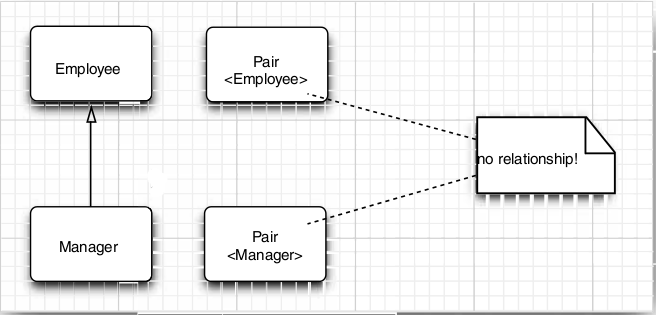
\includegraphics[width=300px,height=200px]{images/relationship.png}
\end{frame}


\section*{Заключение}

\begin{frame}{Заключение}
  \transdissolve
  % Keep the summary *very short*.
  \begin{itemize}
  \item Генеричните типови и методи ни дават
    допълнително ниво на сигурност и
    гъвкавост
   \item Използвайте винаги генеричните версии
    на класовете, ако съществуват такива
   \item Не забравяйте, че в Java generics е
    реализиран на ниво компилатор –
    виртуалната машина, не знае почти
    нищо за генеричните типове
  \end{itemize}
  
  % The following outlook is optional.
  \vskip0pt plus.5fill
  \begin{itemize}
  \item
    Следващият път:
    \begin{itemize}
    \item
      Колекции
    \end{itemize}
  \end{itemize}
\end{frame}

\begin{frame}{Въпроси}
  \transdissolve
  \begin{center}
    \LARGEТук е момента да зададете вашите въпроси! :-)
  \end{center}
\end{frame}

\begin{frame}{Край}
  \transdissolve
  \begin{center}
    \LARGEБлагодаря Ви за вниманието!
  \end{center}
\end{frame}

\end{document}

%%% Local Variables: 
%%% mode: latex
%%% TeX-master: t
%%% End: 
